% Options for packages loaded elsewhere
\PassOptionsToPackage{unicode}{hyperref}
\PassOptionsToPackage{hyphens}{url}
%
\documentclass[
  man]{apa6}
\usepackage{amsmath,amssymb}
\usepackage{lmodern}
\usepackage{iftex}
\ifPDFTeX
  \usepackage[T1]{fontenc}
  \usepackage[utf8]{inputenc}
  \usepackage{textcomp} % provide euro and other symbols
\else % if luatex or xetex
  \usepackage{unicode-math}
  \defaultfontfeatures{Scale=MatchLowercase}
  \defaultfontfeatures[\rmfamily]{Ligatures=TeX,Scale=1}
\fi
% Use upquote if available, for straight quotes in verbatim environments
\IfFileExists{upquote.sty}{\usepackage{upquote}}{}
\IfFileExists{microtype.sty}{% use microtype if available
  \usepackage[]{microtype}
  \UseMicrotypeSet[protrusion]{basicmath} % disable protrusion for tt fonts
}{}
\makeatletter
\@ifundefined{KOMAClassName}{% if non-KOMA class
  \IfFileExists{parskip.sty}{%
    \usepackage{parskip}
  }{% else
    \setlength{\parindent}{0pt}
    \setlength{\parskip}{6pt plus 2pt minus 1pt}}
}{% if KOMA class
  \KOMAoptions{parskip=half}}
\makeatother
\usepackage{xcolor}
\IfFileExists{xurl.sty}{\usepackage{xurl}}{} % add URL line breaks if available
\IfFileExists{bookmark.sty}{\usepackage{bookmark}}{\usepackage{hyperref}}
\hypersetup{
  pdftitle={A Replication of Rothman (2011): L3 syntactic transfer selectivity and typological determinacy: The typological primacy model},
  pdfauthor={Kyle Parrish1},
  pdflang={en-EN},
  pdfkeywords={keywords},
  hidelinks,
  pdfcreator={LaTeX via pandoc}}
\urlstyle{same} % disable monospaced font for URLs
\usepackage{graphicx}
\makeatletter
\def\maxwidth{\ifdim\Gin@nat@width>\linewidth\linewidth\else\Gin@nat@width\fi}
\def\maxheight{\ifdim\Gin@nat@height>\textheight\textheight\else\Gin@nat@height\fi}
\makeatother
% Scale images if necessary, so that they will not overflow the page
% margins by default, and it is still possible to overwrite the defaults
% using explicit options in \includegraphics[width, height, ...]{}
\setkeys{Gin}{width=\maxwidth,height=\maxheight,keepaspectratio}
% Set default figure placement to htbp
\makeatletter
\def\fps@figure{htbp}
\makeatother
\setlength{\emergencystretch}{3em} % prevent overfull lines
\providecommand{\tightlist}{%
  \setlength{\itemsep}{0pt}\setlength{\parskip}{0pt}}
\setcounter{secnumdepth}{-\maxdimen} % remove section numbering
% Make \paragraph and \subparagraph free-standing
\ifx\paragraph\undefined\else
  \let\oldparagraph\paragraph
  \renewcommand{\paragraph}[1]{\oldparagraph{#1}\mbox{}}
\fi
\ifx\subparagraph\undefined\else
  \let\oldsubparagraph\subparagraph
  \renewcommand{\subparagraph}[1]{\oldsubparagraph{#1}\mbox{}}
\fi
\newlength{\cslhangindent}
\setlength{\cslhangindent}{1.5em}
\newlength{\csllabelwidth}
\setlength{\csllabelwidth}{3em}
\newlength{\cslentryspacingunit} % times entry-spacing
\setlength{\cslentryspacingunit}{\parskip}
\newenvironment{CSLReferences}[2] % #1 hanging-ident, #2 entry spacing
 {% don't indent paragraphs
  \setlength{\parindent}{0pt}
  % turn on hanging indent if param 1 is 1
  \ifodd #1
  \let\oldpar\par
  \def\par{\hangindent=\cslhangindent\oldpar}
  \fi
  % set entry spacing
  \setlength{\parskip}{#2\cslentryspacingunit}
 }%
 {}
\usepackage{calc}
\newcommand{\CSLBlock}[1]{#1\hfill\break}
\newcommand{\CSLLeftMargin}[1]{\parbox[t]{\csllabelwidth}{#1}}
\newcommand{\CSLRightInline}[1]{\parbox[t]{\linewidth - \csllabelwidth}{#1}\break}
\newcommand{\CSLIndent}[1]{\hspace{\cslhangindent}#1}
\ifLuaTeX
\usepackage[bidi=basic]{babel}
\else
\usepackage[bidi=default]{babel}
\fi
\babelprovide[main,import]{english}
% get rid of language-specific shorthands (see #6817):
\let\LanguageShortHands\languageshorthands
\def\languageshorthands#1{}
% Manuscript styling
\usepackage{upgreek}
\captionsetup{font=singlespacing,justification=justified}

% Table formatting
\usepackage{longtable}
\usepackage{lscape}
% \usepackage[counterclockwise]{rotating}   % Landscape page setup for large tables
\usepackage{multirow}		% Table styling
\usepackage{tabularx}		% Control Column width
\usepackage[flushleft]{threeparttable}	% Allows for three part tables with a specified notes section
\usepackage{threeparttablex}            % Lets threeparttable work with longtable

% Create new environments so endfloat can handle them
% \newenvironment{ltable}
%   {\begin{landscape}\centering\begin{threeparttable}}
%   {\end{threeparttable}\end{landscape}}
\newenvironment{lltable}{\begin{landscape}\centering\begin{ThreePartTable}}{\end{ThreePartTable}\end{landscape}}

% Enables adjusting longtable caption width to table width
% Solution found at http://golatex.de/longtable-mit-caption-so-breit-wie-die-tabelle-t15767.html
\makeatletter
\newcommand\LastLTentrywidth{1em}
\newlength\longtablewidth
\setlength{\longtablewidth}{1in}
\newcommand{\getlongtablewidth}{\begingroup \ifcsname LT@\roman{LT@tables}\endcsname \global\longtablewidth=0pt \renewcommand{\LT@entry}[2]{\global\advance\longtablewidth by ##2\relax\gdef\LastLTentrywidth{##2}}\@nameuse{LT@\roman{LT@tables}} \fi \endgroup}

% \setlength{\parindent}{0.5in}
% \setlength{\parskip}{0pt plus 0pt minus 0pt}

% Overwrite redefinition of paragraph and subparagraph by the default LaTeX template
% See https://github.com/crsh/papaja/issues/292
\makeatletter
\renewcommand{\paragraph}{\@startsection{paragraph}{4}{\parindent}%
  {0\baselineskip \@plus 0.2ex \@minus 0.2ex}%
  {-1em}%
  {\normalfont\normalsize\bfseries\itshape\typesectitle}}

\renewcommand{\subparagraph}[1]{\@startsection{subparagraph}{5}{1em}%
  {0\baselineskip \@plus 0.2ex \@minus 0.2ex}%
  {-\z@\relax}%
  {\normalfont\normalsize\itshape\hspace{\parindent}{#1}\textit{\addperi}}{\relax}}
\makeatother

% \usepackage{etoolbox}
\makeatletter
\patchcmd{\HyOrg@maketitle}
  {\section{\normalfont\normalsize\abstractname}}
  {\section*{\normalfont\normalsize\abstractname}}
  {}{\typeout{Failed to patch abstract.}}
\patchcmd{\HyOrg@maketitle}
  {\section{\protect\normalfont{\@title}}}
  {\section*{\protect\normalfont{\@title}}}
  {}{\typeout{Failed to patch title.}}
\makeatother

\usepackage{xpatch}
\makeatletter
\xapptocmd\appendix
  {\xapptocmd\section
    {\addcontentsline{toc}{section}{\appendixname\ifoneappendix\else~\theappendix\fi\\: #1}}
    {}{\InnerPatchFailed}%
  }
{}{\PatchFailed}
\keywords{keywords\newline\indent Word count: X}
\DeclareDelayedFloatFlavor{ThreePartTable}{table}
\DeclareDelayedFloatFlavor{lltable}{table}
\DeclareDelayedFloatFlavor*{longtable}{table}
\makeatletter
\renewcommand{\efloat@iwrite}[1]{\immediate\expandafter\protected@write\csname efloat@post#1\endcsname{}}
\makeatother
\usepackage{lineno}

\linenumbers
\usepackage{csquotes}
\ifLuaTeX
  \usepackage{selnolig}  % disable illegal ligatures
\fi

\title{A Replication of Rothman (2011): L3 syntactic transfer selectivity and typological determinacy: The typological primacy model}
\author{Kyle Parrish\textsuperscript{1}}
\date{}


\shorttitle{Rothman (2011) Replication}

\authornote{

Add complete departmental affiliations for each author here. Each new line herein must be indented, like this line.

Enter author note here.

Correspondence concerning this article should be addressed to Kyle Parrish, 15 Seminary Place, New Brunswick, NJ. E-mail: \href{mailto:kyle.parrish@rutgers.edu}{\nolinkurl{kyle.parrish@rutgers.edu}}

}

\affiliation{\vspace{0.5cm}\textsuperscript{1} Rutgers University}

\abstract{%
One or two sentences providing a \textbf{basic introduction} to the field, comprehensible to a scientist in any discipline.

Two to three sentences of \textbf{more detailed background}, comprehensible to scientists in related disciplines.

One sentence clearly stating the \textbf{general problem} being addressed by this particular study.

One sentence summarizing the main result (with the words ``\textbf{here we show}'' or their equivalent).

Two or three sentences explaining what the \textbf{main result} reveals in direct comparison to what was thought to be the case previously, or how the main result adds to previous knowledge.

One or two sentences to put the results into a more \textbf{general context}.

Two or three sentences to provide a \textbf{broader perspective}, readily comprehensible to a scientist in any discipline.
}



\begin{document}
\maketitle

The distinction between third language (L3) and second language (L2) learning in adulthood has received a significant increase in research over the last 15 years.
One key difference between L3 and L2 learning is that third language learners can be influenced by two languages during the process of acquisition, rather than just their native language as is the case in L2 learning.
However, there is not a consensus how exactly and if L3 learners are impacted by their two known languages.
Guided by empirical research, several models have been proposed to predict how the L1 and L2 will impact L3 learning and acquisition.
One of the first models suggested that L3 learners could draw on either their first or second language, and that this influence would be helpful (The Cumulative Enhancement Model; (\textbf{flynn?})).
Others predict that the L2 has a privileged status and inhibits access to the L1 (the L2 Status Factor; Bardel \& Falk), or, oppositely, that the native language has a special status (Hermas, 2010).
Finally, another set of models suggest that structural similarity between the learned language and background language(s) predicts influence.
The Typological Primacy Model (TPM) predicts that wholesale (one entire language) transfer occurs to the L3 at some point during the ``initial stages'' of L3 development.
The language which transfers, either the L1 or the L2, is determined by the individual on the basis of input, but is generally predicted to be the language that is structurally closer to the L3 (e.g., Spanish, not English, would transfer to L3 Brazilian Portuguese).
The Linguistic Proximity Model (LPM) also posits that structural similarity plays a key role predicting how the L1 or L2 influence the L3, but suggests that this happens in a property-by-property basis, rather than all at once.
These various predictions have each received some support in the literature. In a recent systematic review, (\textbf{rothman?})/(\textbf{puig?}) reviewed 92 total L3 studies, aiming to aggregate the evidence for each model.
The results showed that, while each model had some empirical support, most studies could be explained by Typological transfer as predicted by the TPM.
Many studies also were potentially explained, however, by L2 status effects.
It is important to note that many of these studies were coded as providing evidence simultaneously for two views.
That is, a single study which reported L2 influence on the L3 was coded as both L2 and typological influence, since they could not demonstrate that the influence in the L3 was due to L2 status and not structural similarity.

In order to avoid this confound, it has been suggested that L3 studies utilize a so-called mirror-image group design.
The mirror image design, proposed in ((\textbf{foote?}), Rothman 2010), recruits two groups that speak the same L3, and same background languages, but their order of acquisiion is reversed for the L1 and L2 (e.g.~L1 Spanish-L2 English-L3 BP, L1 English-L2 Spanish-L3 BP).
By comparing the L3 of these groups, distinct performance on a given experimental task would provide evidence that order of acquisition is an important predictor in predicting how background languages influence a third language.
On the other hand, if the groups perform similarly and L2 proficiency is taken into account, it would be evidence that having the same background languages, regardless of their order of acquisition, would predict L3 transfer.

One of the first studies to utilize this mirror image design was Rothman (2011).
In the study, two L3 groups, (L1 Italian-L2 English-L3 Spanish and L1 English-L2 Spanish-L3 Brazilian Portuguese) along with a Spanish native and Brazilian Portuguese native group, completed two tasks which measured their judgment of determiner phrase noun-adjective combinations.
In Spanish, Italian, and Portuguese, adjectives can appear in pre-nominal or post-nominal position and constitute a change in meaning.
Figure \emph{mark} from Rothman (2011) provides an example; post-nominal adjectives induce a set-denoting interpretation, while pre-nominal adjectives elicit a kind-denoting interpretation.
English, on the other hand, does not distinguish kind and set denotation syntactically, as the adjective appears pre-nominally in both bases.
The results of both tasks revealed that all four groups similarly judged sentences given to them in either their L3 or L1 (for the native groups).
This was taken as evidence that, since one group's had this feature and the other group's L2 had the L3 features, that the structural similarity of these languages, rather than the order of acquisition, predicted L3 transfer.

\hypertarget{the-present-study}{%
\section{The present study}\label{the-present-study}}

The present study is a conceptual replication of Rothman (2011), in which the original methods and analysis were intended to be replicated in a similar population of L3 learners.
This replication re-created similar stimuli using the available examples from the original study, and other similar studies that used the same type of tasks (cites), and measured L2 and L3 proficiency using the LexTALE, rather than a cloze and grammar test.

The rationale for this replication is its importance and impact on the field of L3 acquisition over the last decade and would have implications for both supporters of the TPM and other models.
In the event that a difference is found between L3 groups, the basis for the model itself could be called into question in favor of other models.
This finding would call into question whether the TPM can be considered the dominant or most accurate model in L3 acquisition, given that the recent systematic review (Rothman et al., 2019) concluded that typological transfer accounted for most outcomes in L3 morphosyntax, rather than order of acquisition.
However, many of these studies' designs and statistical analyses only allow for binary interpretation of the results.
That is, the design of these studies is such that either the L3 is impacted by the L1 or the L2, rather than allowing for the combination of both languages to impact the L3.
This strategy is present in many L3 studies and is arguably influenced by Rothman (2011).
A failed replication of this study would not only call into question its own findings, but findings in many other studies which adopted similar methodology and now serve as the empirical basis to the TPM.
On the other hand, a successful replication of Rothman (2011) would suggest that full influence is possible and would strengthen the basis of the TPM and lessen counter arguments that include potential sampling issues, while also quantifying the (un)certainty related to this similar performance between groups.

\hypertarget{methods}{%
\section{Methods}\label{methods}}

We report how we determined our sample size, all data exclusions (if any), all manipulations, and all measures in the study.

\hypertarget{participants}{%
\subsection{Participants}\label{participants}}

A total of 202 participants took part in this experiment, consisting of 4 total groups.
The first two groups were L3 speakers of Portuguese who spoke L1 English-L2 Spanish (n = 12; henceforth the L1 English group) and L1 Spanish-L2 English (n = 60; henceforth the L1 English group).
Additionally, a group of Portuguese native speakers (n = 61) and a group of Spanish native speakers (69) also participated.

\hypertarget{materials}{%
\subsection{Materials}\label{materials}}

Two tasks were given to participants

\hypertarget{semantic-interpretation-task}{%
\subsubsection{Semantic interpretation task}\label{semantic-interpretation-task}}

This task was designed to evaluate how the adjective's position in a DP (pre or post nominal) impacted meaning in both the L2 and L3.
The task had both a Spanish and Brazilian Portuguese version, in which 5 target items were tested in each of a pre-nominal and post-nominal condition.
Equal numbers of fillers were used which tested other properties (e.g., anaphora resolution) used in subsequent studies.
Below is an example taken of the Semantic interpretation task in Spanish taken directly from Rothman (2011).

\textbf{Prompt}
``Los maridos honestos se merecen el respeto de sus mujeres.''

\textbf{Answer choices}

a.) \emph{De todos los maridos que hay solo algunos, los que son honestos merecen el respeto de sus esposas.}

b.) Todo marido se merece el respeto de su esposa porque todo marido es, por ser marido, honesto.

\textbf{Prompt}
``Los valientes Incas tenían mucho éxito.''

\textbf{Answer choices}

a.) Entre los incas había los valientes y los no valientes, así que todo inca que era valiente también tenía éxito

b.) \emph{Ser Inca equivale a ser valiente, así que todo Inca tenía éxito.}

\hypertarget{context-based-collocation-task}{%
\subsubsection{Context-based Collocation Task}\label{context-based-collocation-task}}

A second task elicited production of adjectival DPs by way of context.
In the task, participants read a short story and had to fill in a blank at the end of the story with either a pre or post nominal adjective.
Below is an example of the Context-based Collocation Task in Spanish taken directly from Rothman (2011).

\emph{Example}

Mi esposa se llama Magda. Ella es una persona muy amable y cariñosa. Aunque solo tenemos 22 años, hace mucho tiempo que somos amigas. Magda es una vieja amiga \_\_\_\_\_\_\_ (viejo).

`My best friend is named Magda. She is a very nice and affectionate person. Even though we are only 22-years-old, we have been friends for a long time. Magda is an old friend.''

\hypertarget{procedure}{%
\subsection{Procedure}\label{procedure}}

\hypertarget{statistical-analysis}{%
\subsection{Statistical analysis}\label{statistical-analysis}}

Two sets of analyses were carried out, a replication of the analysis of the original study and a second analysis using a Bayesian approach.
The original study used two-way ANOVAs for each of the two tasks (the Semantic interpretation and context-based collocation tasks).
In each model, the number of correct responses was analyzed as a function of item type (preposed or postposed), group and their interaction.

A. Why Bayesian. If the audience requires it, explain what benefits will be gleaned by a Bayesian analysis (as opposed to a frequentist analysis).
B. Goals of analysis. Explain the goals of the analysis. This prepares the audience for the type of models to expect and how the results will be described.

The goal of the Bayesian analysis was to determine whether there were differences between the probability of a correct response by each group while taking preposed and postposed positions into account.
One advantage of a Bayesian approach is the ability to provide evidence for practical equivalence or estimate differences.

For the Bayesian analysis, two logistic multilevel regression models analyzed the probability of answering a given trial correctly as a function of group, item type, and their interaction for each task.
\emph{Random intercepts for item and participant were also included.}
The models was run using with 4000 iterations of Hamiltonian Monte-Carlo sampling (1000 warm up), across 4 chains and 8 processing cores.

\hypertarget{results}{%
\section{Results}\label{results}}

\ref{fig:cmc-desc} shows the average correct responses (out of 5) for the Context-based collocation task by all 4 groups.

\begin{figure}
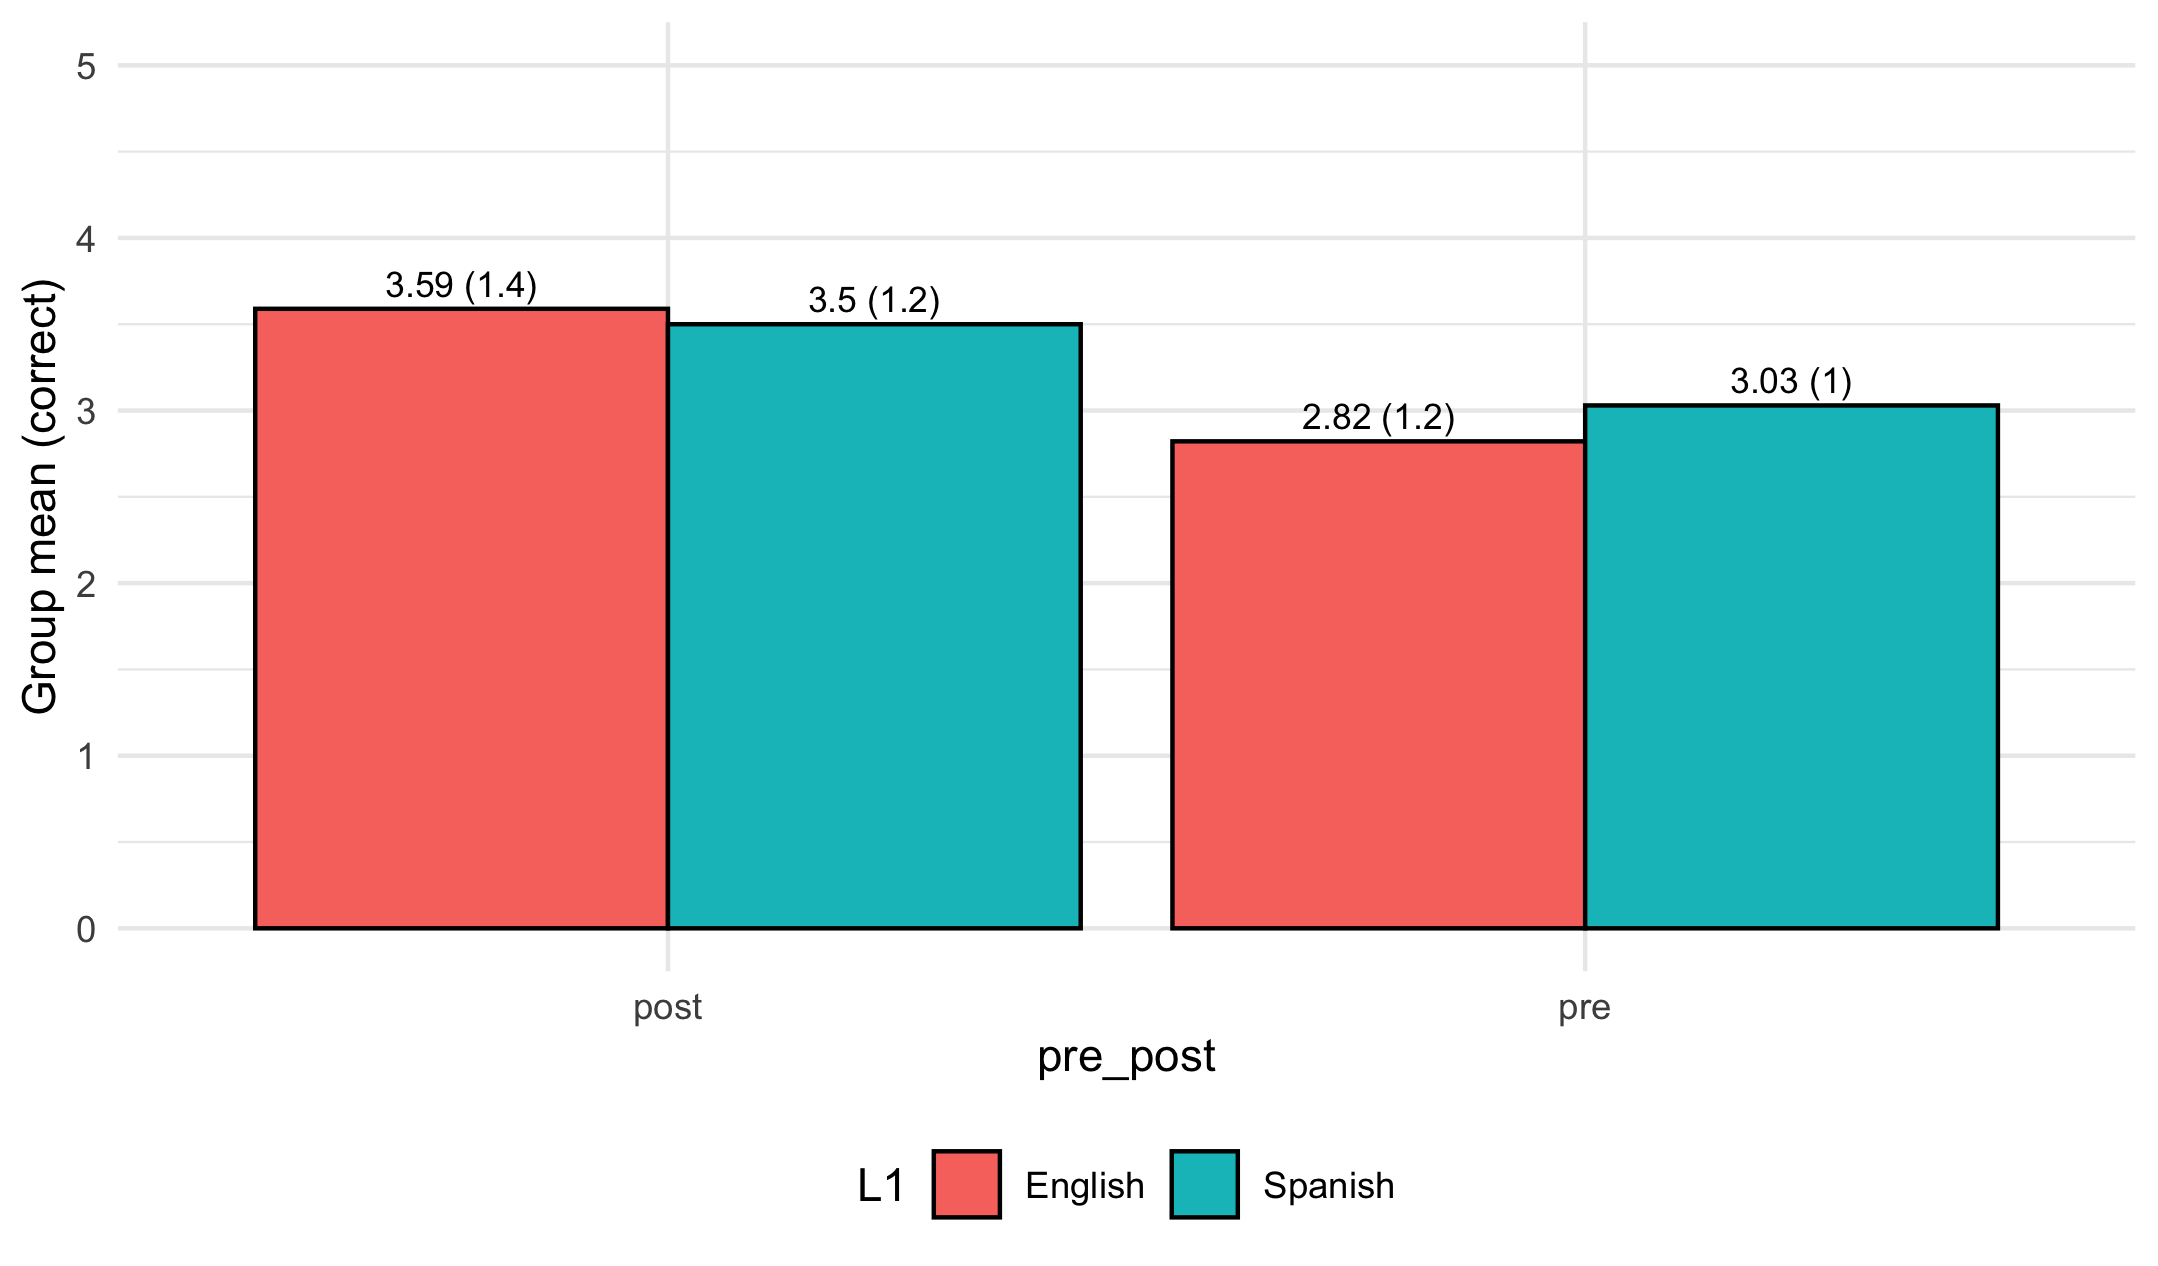
\includegraphics[width=7in]{figs/cbc_desc} \caption{Context-based Collocation Task}\label{fig:cmc-desc}
\end{figure}

\ref{fig:sem-desc} shows the average correct responses (out of 5) for the Context-based collocation task by all 4 groups.

\begin{figure}
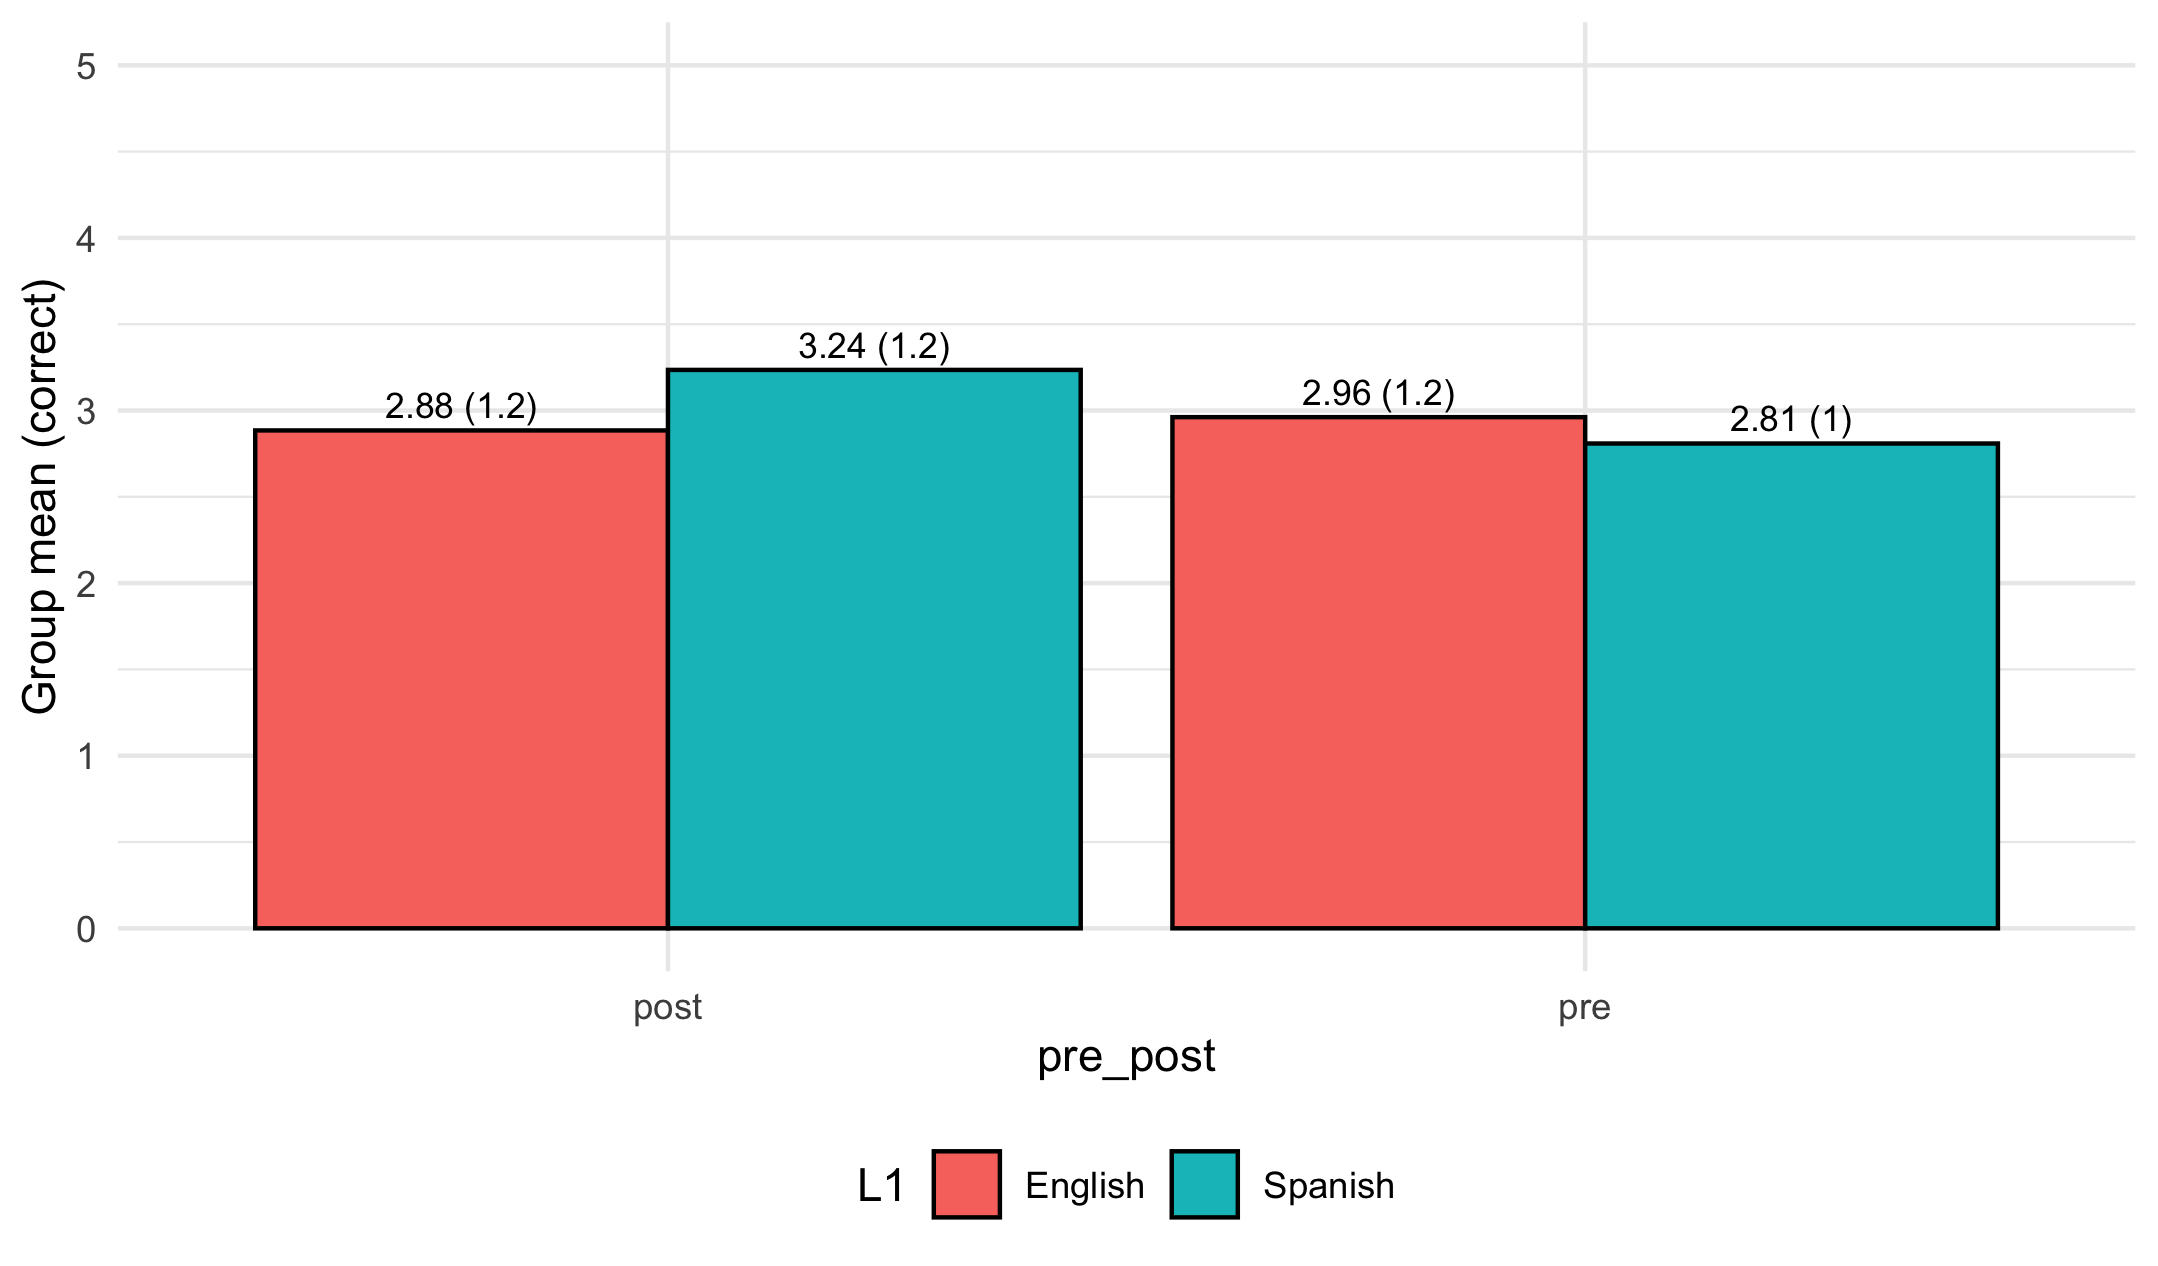
\includegraphics[width=7in]{figs/semantic_desc} \caption{Semantic Interpretation Task}\label{fig:sem-desc}
\end{figure}

\hypertarget{discussion}{%
\section{Discussion}\label{discussion}}

Overall, the present study failed to replicate the null results reported in Rothman (2011).
In particular, the L3 groups performed differently in the present study on both the semantic interpretation and the collocation collocation tasks.
Interestingly, the Spanish bilingual group answered correctly less often than the Spanish native group in both conditions in the semantic interpretation task and in the post-nominal condition for the context-based collocation task.
One possible explanation for this finding is that their L2, English, influenced their judgments of meaning in their L3.
This result would best be explained by the L2 status factor, which predicts that the L2 influences the L3 while inhibiting access to the L1.

Just as in the original study, these results do not necessarily demonstrate that transfer is not property by property, since only a single property was tested.

These results could not be explained by the TPM, differently from the original study.
A few key differences seem readily apparent between this data and Rothman (2011).
First, the mean number of correct answers in Rothman (2011) was over 4 out of 5, which suggests that it is possible that a ceiling effect could explain the similarity between groups.
In other words, the stimuli used in the study might have been easily interpreted by the participants and been a result of their acquisition of the property in BP, rather than influence from Spanish.
sampling
Another possibility is sampling error - the original study had 60 total participants across 4 groups.
While the statistical power and risk for sampling error cannot be calculated using the data reported in the study, it is arguable that this sample is not representative of the population it is intended to represent.
The present study, on the other hand, carried out a power analysis and found that \textbf{power analysis}.

These results call into question whether, in addition to this study, other studies in L3A similar issues relating to statistical power might be at play.
In particular, low sample size (under-powered) studies have a high risk of producing a false negative finding.
Figure \ref{fig:pa} demonstrates this issue by using simulated data.
In particular, small, medium and large effects are simulated.
The figure shows that, unless the effect is very large, the probability of a false negative can be higher than any significant result being found in the data.

\begin{figure}
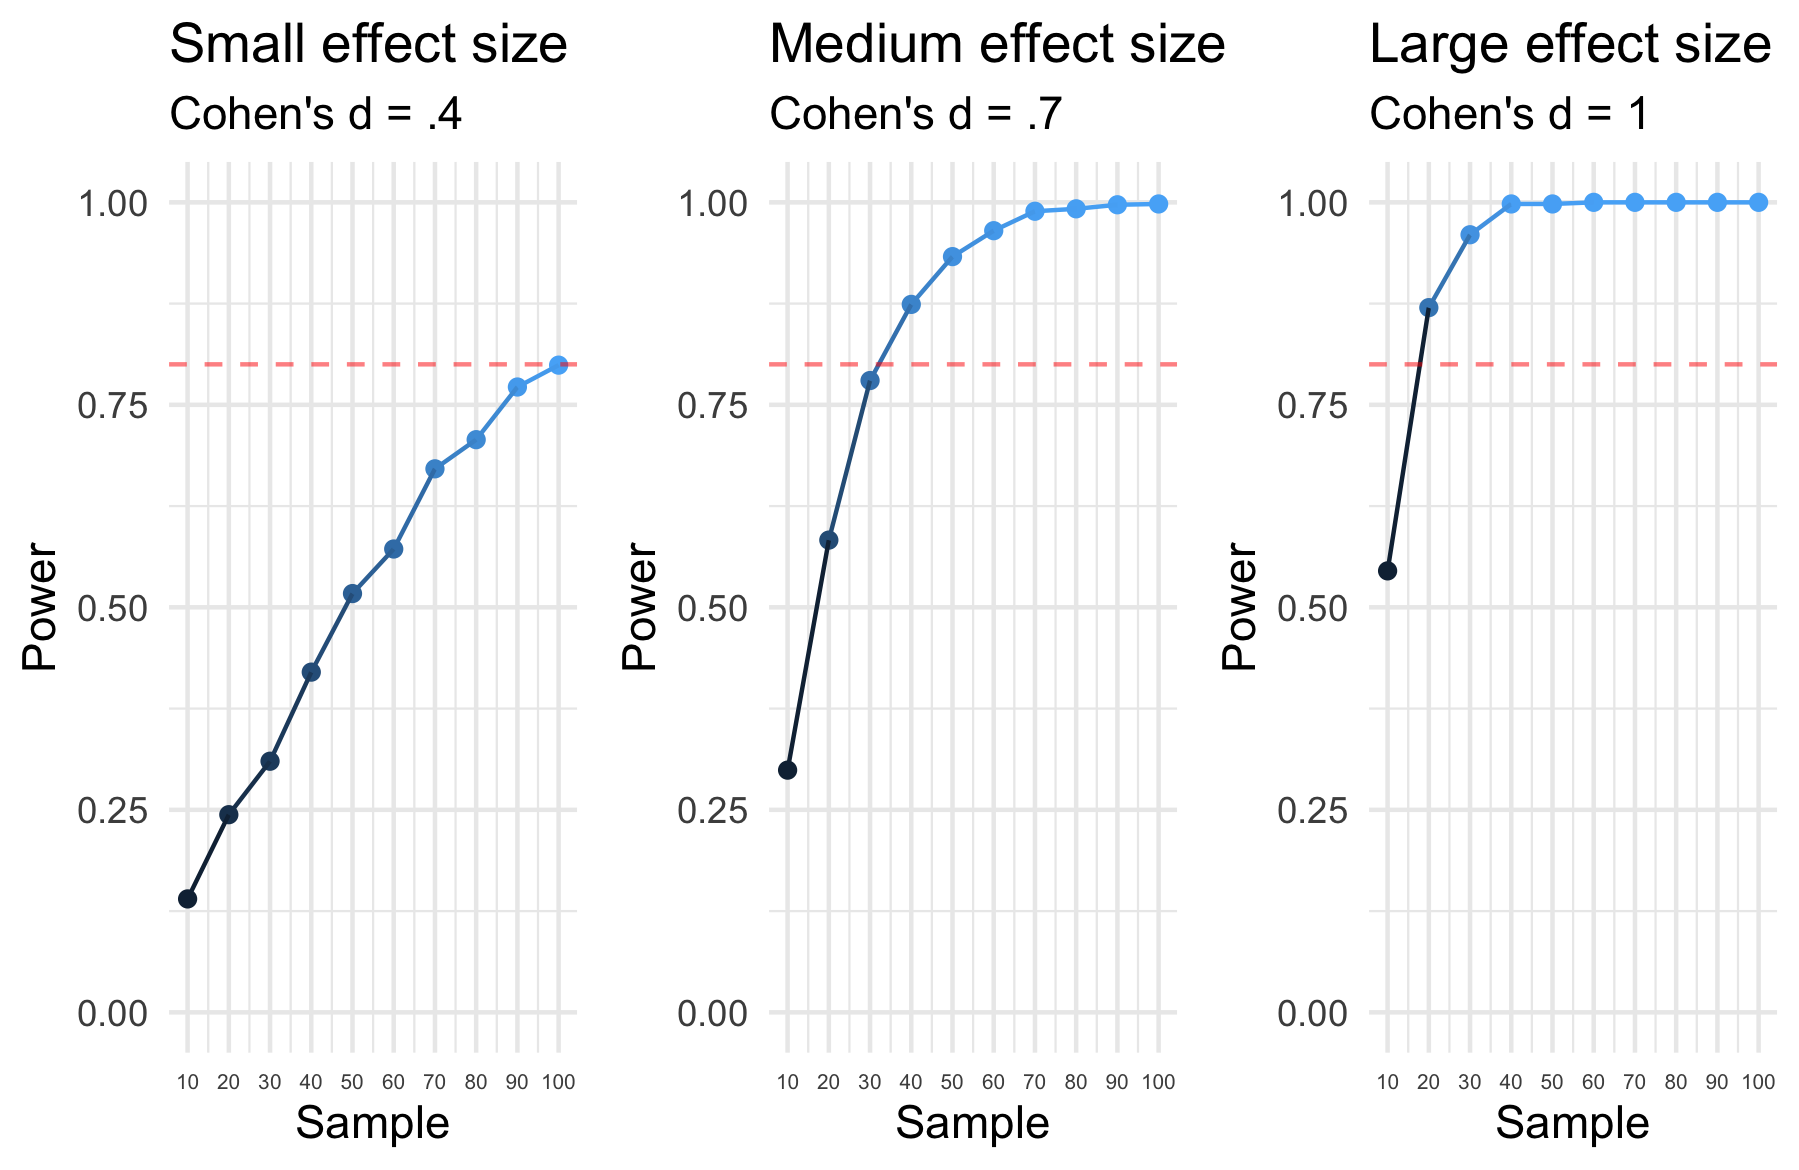
\includegraphics[width=6in]{figs/power_curve} \caption{Power Analyses for small, medium and large effect sizes}\label{fig:pa}
\end{figure}

Additionally, the so-called ``winners curse'' (cite) is an issue with low sample studies.
That is, even when an effect is found in an underpowered study, it is very likely over-estimated.
Figure \ref{fig:sim} shows this, again using simulated data.
Overall, 2000 simulations were carried out.

\begin{figure}
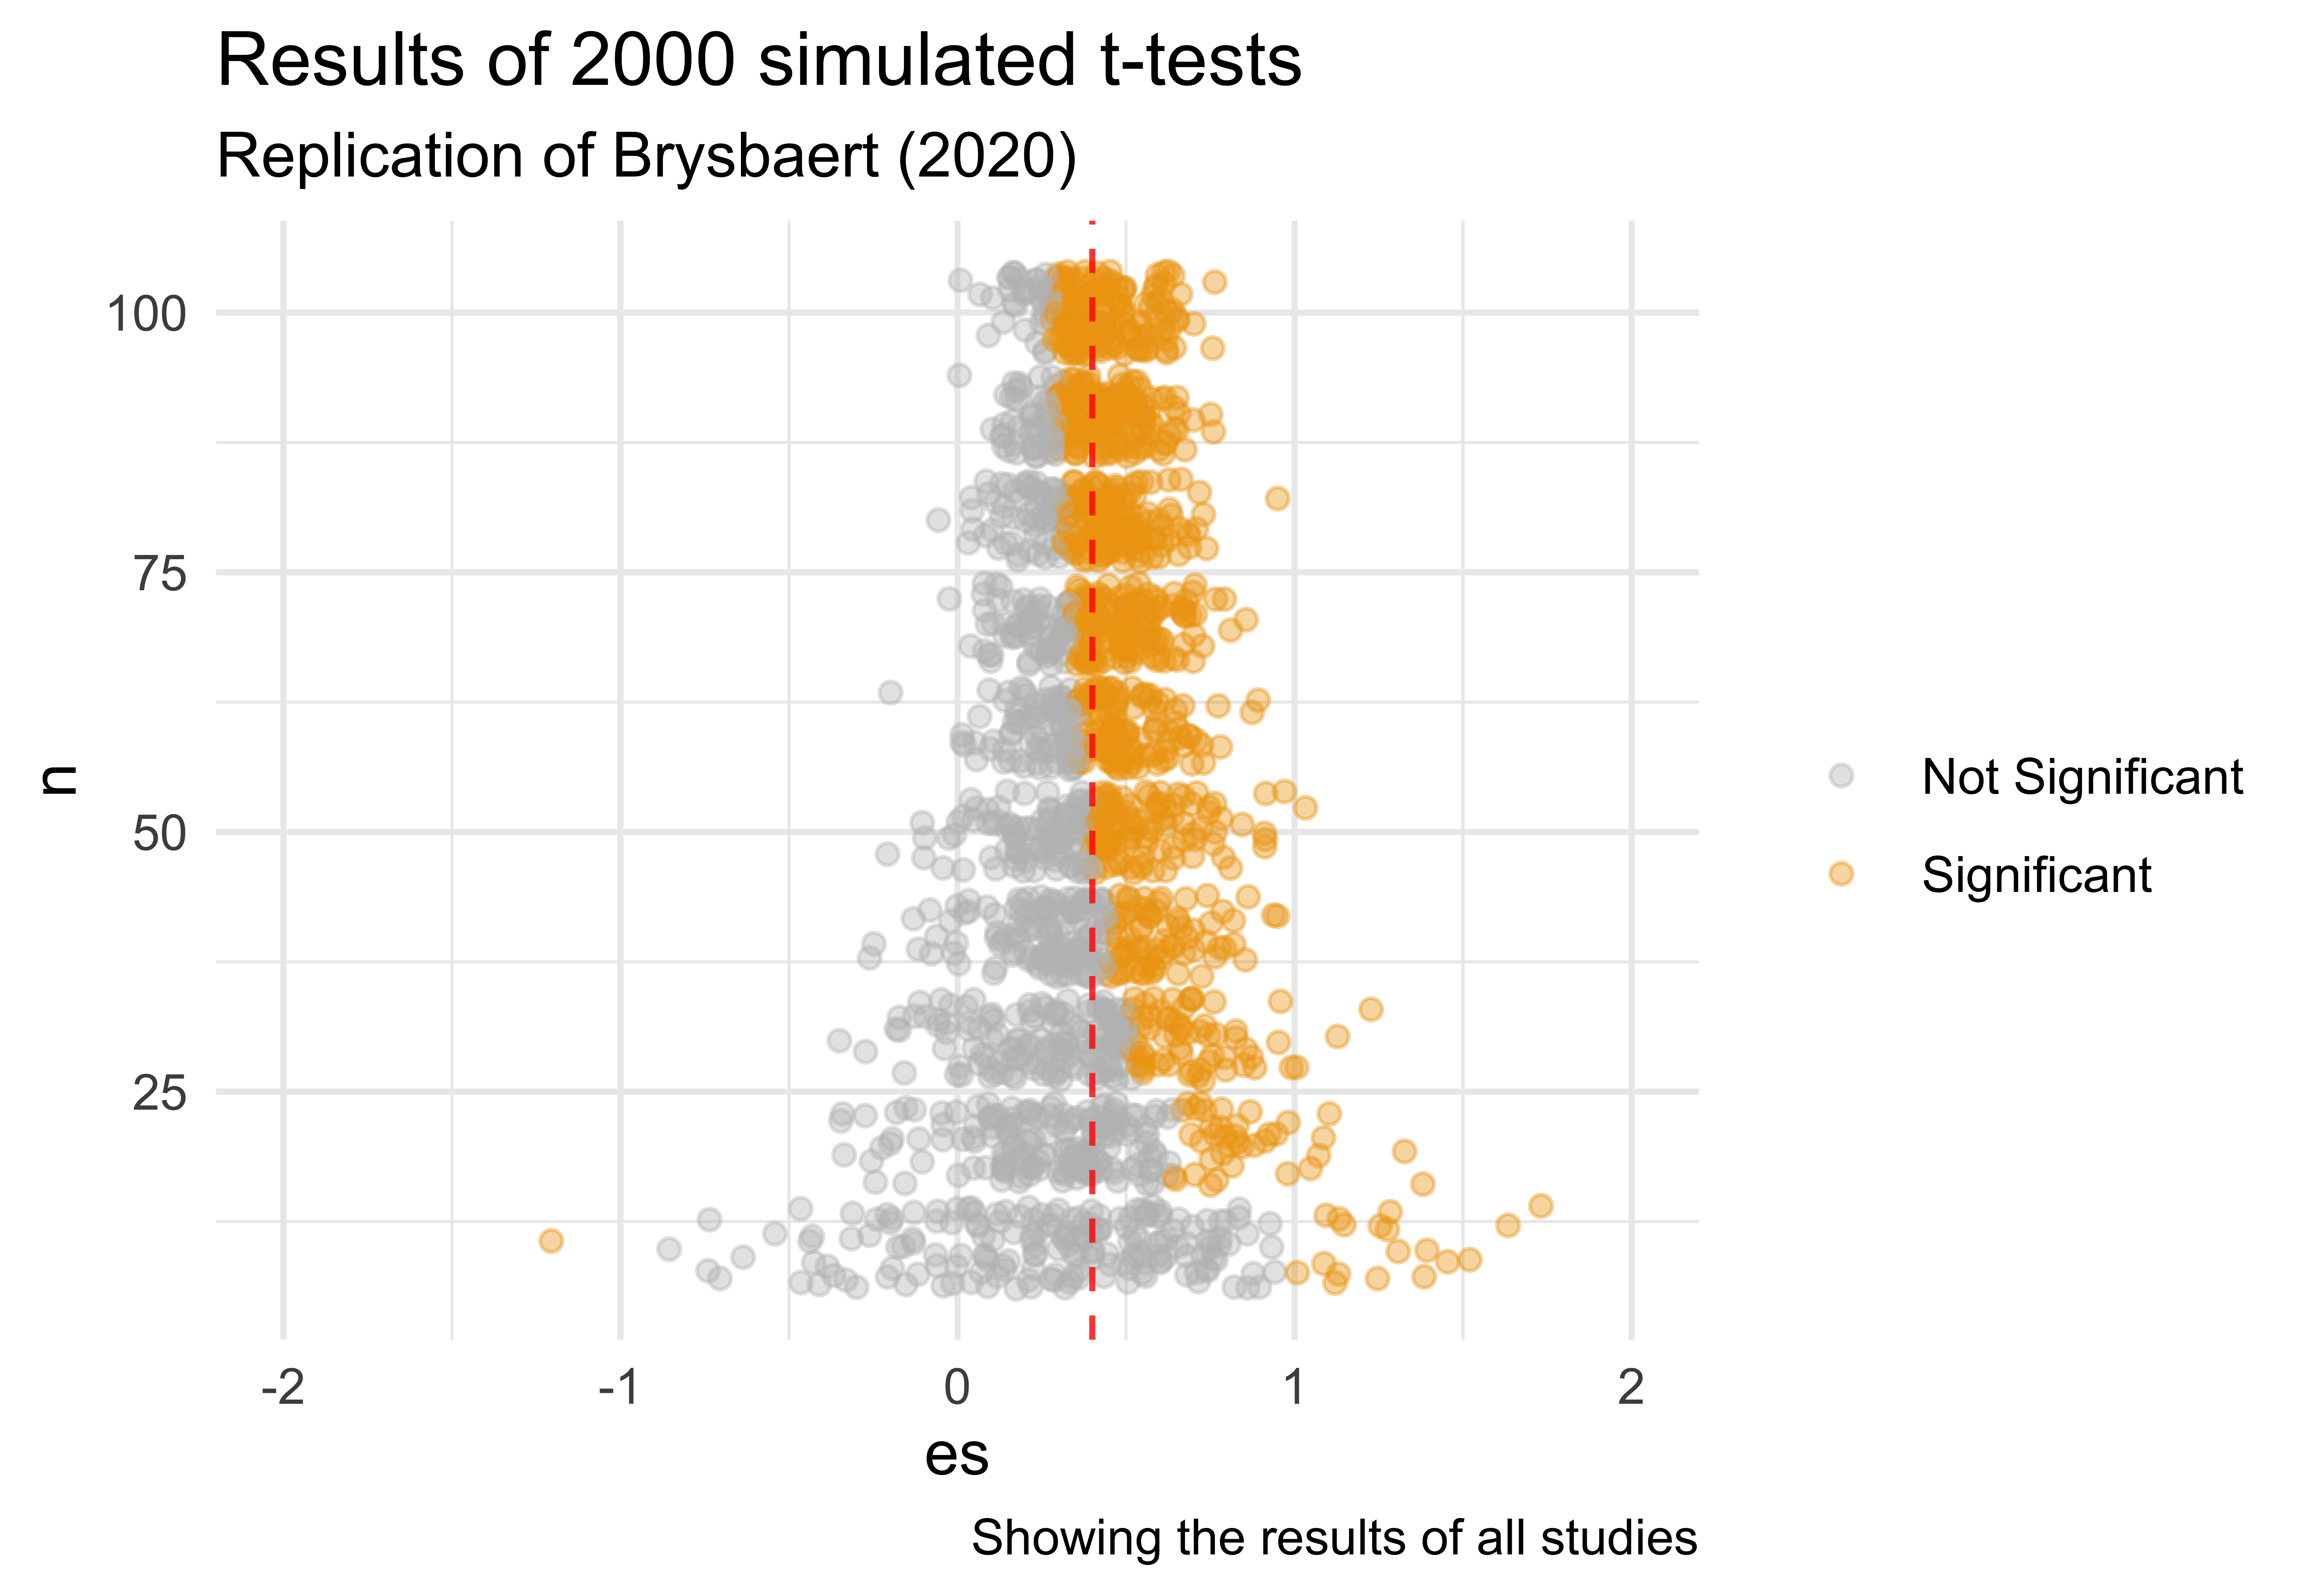
\includegraphics[width=22.55in]{figs/2k_sim_all} \caption{Results from 2000 simulated t-tests}\label{fig:sim}
\end{figure}

\newpage

\hypertarget{references}{%
\section{References}\label{references}}

\begingroup
\setlength{\parindent}{-0.5in}
\setlength{\leftskip}{0.5in}

\hypertarget{refs}{}
\begin{CSLReferences}{0}{0}
\end{CSLReferences}

\endgroup


\end{document}
